%!TEX root = ../report_template.tex
\section*{Methods}
%Todo: Think about citations



\textbf{The Pearson correlation coefficient} \cite{rodgers_thirteen_1988}, denoted as $r$, is a statistical measure used to assess the linear relationship between two sets of data, $X$ and $Y$. It is computed as the ratio of the sample covariance of the $X$ and $Y$ to the product of their sample standard deviations:
\begin{equation}
    r = \frac{\sum_{i=1}^n (X_i - \overline{X}) (Y_i - \overline{Y})}{\sqrt{\sum_{i=1}^n(X_i-\overline{X})^2 \cdot \sum_{i=1}^n(Y_i-\overline{Y})^2}}
\end{equation}


\paragraph{Datasets:}

% Maybe move it later
\begin{figure*}[t!]
    \centering
    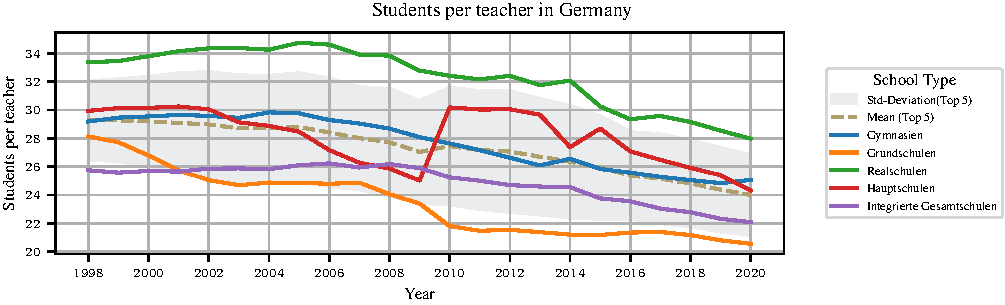
\includegraphics{fig/fig_students_per_teacher_per_school_type.pdf}
    \caption{Students-to-teacher ratio of the five most common school types in Germany. The ratio of full- and part-time teachers is displayed foreach school type and aggregated to their mean (\textcolor{TUgold}{\rule[-0.2ex]{0.5em}{2pt} \rule[-0.2ex]{0.5em}{2pt}}) and standard deviation (\textcolor{TUgray}{\rule[-0.2ex]{1em}{0.8em}}).}
    \label{fig:spt-type}
\end{figure*}

The datasets used in this paper can be grouped into causes and effects. Therefore, the causes are societal, demographic, or political factors influencing the quality of the German school system. This could be the number of students, teachers, or budget provided by the German government. In contrast, this paper defines the effects of the causes as observable measures of the students' performance. Examples are the average grades, PISA study results, or the rate of repeaters and school-leavers.

% Causes
The first cause dataset is provided in the \textit{Fachreport Schuljahr 2020/21} of the \citeauthor{statistische_bundesamt_allgemeinbildende_2022} and contains the number of teachers from 1992 until 2020. The dataset groups them primarily according to their contract type, federal state, and school type. This paper merges the teacher counts with two student datasets, which are published in the \textit{Genesis} database of the \citeauthor{statistische_bundesamt_statistisches_2023}. Both provide the number of children as different groupings and aggregations. The first contains the number of children per grade and school type  for the years 1998 to 2022. In contrast, the second table provides the absolute amount of children, leavers, and beginners in each federal state from 1997 to 2022. Therefore, the analysis of the merged dataset can only be conducted separately for school types and federal states.

To conclude the causes, this paper introduces the budget per child, which is provided in the \textit{Genesis} database of the \citeauthor{statistische_bundesamt_statistisches_2023}. The dataset contains the budget per child for the years 2010 to 2022 and is grouped by federal states. In contrast to the demographic and societal causes above, the budget models a direct political factor. To adjust the budget to inflation, it is multiplied with the \textit{Verbraucherpreisindex} relative to 2022 provided by the \citeauthor{statistische_bundesamt_statistisches_2023}. 


% Effects
Moreover, the primary effects on students' performance are the basis for the analysis of the German school system. One of the few publicly available datasets containing grades is the average Abitur grades per federal state. The grades are published every year by the \citeauthor{kultusminister_konferenz_abiturnoten_nodate}. Each file contains the count of children per written grade and federal state. In addition, the grades are defined in $0.1$ steps, with $4.0$ as the worst and $1.0$ as the best grade. Furthermore, the amount of children who failed with a grade worse than $4.0$ is aggregated in an additional column. 

Although this is a great model for the performance of children attending grammar schools, a general performance measure for all school types is required. Accordingly, this paper uses the number of repeaters derived from the \textit{{GENESIS}} Database of the \citeauthor{statistische_bundesamt_statistisches_2023}. There, the absolute count of repeaters by federal state, school type, and year is provided for the years 1998 to 2022.

% Say that also other effects such as people without degree, special educational needs were also explored but don't have a big impact due to their low percentage relative to all schoolchildren

\paragraph{First trends and basic analysis}
% Todo: Better Introduction

Having introduced all used datasets, this paragraph aims to investigate potential patterns through an exploratory data analysis of the potential causes and effects. 

% Describe causes
% Todo: Sources
Firstly, regard the demographic effects on the number of children attending school and teachers employed by school type and federal state. The exploratory data analysis has shown that the number of schoolchildren decreases steadily from 1998 to 2014. Instead, it increased from 2019 to 2022 because more children started their education and fewer left school. Furthermore, more children graduate from grammar schools with university entrance qualifications. This demographic effect is combined with an increasing number of teachers across all German school types and federal states. Although, the percentage of part-time teachers is increasing, the number of full-time teachers is decreasing until 2020.

Given the hypothesis that having more teachers per student increases the quality of teaching, the datasets can be merged. As already explained, this merge can only been done separately for school types and federal states. Furthermore, the student-to-teacher ratio is calculated over all full- and part-time teachers, since they represent the majority ({\raise.17ex\hbox{$\scriptstyle\mathtt{\sim}$}} $90\%$) of the distribution. In contrast, the teachers who are employed on an hourly basis are excluded due to their small impact on the teaching quality and sparse representation in the data. The results (\autoref{fig:spt-type}) show that from 1998 to 2020, the ratio decreased for the five most common school types. As a result, the average decreases from 29 to 24 children per teacher. Together with the hypothesis, it follows that the quality of teaching should increase, and thus the performance measures should increase.

Besides the demographic measures, the federal states plan their school budgets independently (TODO source). The analysis of the adjusted budget to inflation per child has shown that it steadily increases for all federal states. Although, this may be caused by the increasing number of teachers and the goals of digitalization at schools (TODO source).

% Effects

Now that the basic effects that may influence the students' performance have been identified, it is possible to study the performance measures. As the analysis of the students datasets has shown, more children are attending grammar schools in Germany. Thus, the average Abitur grade of the children is a great measure of the performance of many children. \autoref{fig:rising-grades} shows that the average grades are increasing in all federal states. Furthermore, a linear regression can be employed to represent their mean. Importantly, the regression is calculated on the data before 2021 because of the COVID-19 pandemic beginning in 2020. In 2022, the grades significantly increased compared to the years before the pandemic. This could indicate that the pandemic has had novel consequences for the educational system. Due to the lack of data following the pandemic, this paper will solely focus on the linear trend until 2020. Furthermore, an additional analysis of the relative number of failed students has shown that the failure rate has no repetitive or linear pattern. Therefore, the provided results in \autoref{fig:rising-grades} are only valid for children graduating with a grade of at least 4.0.

\begin{figure}[h]
    \centering
    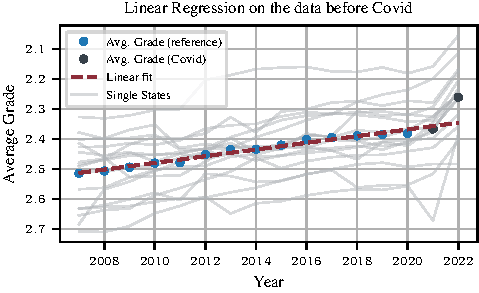
\includegraphics{fig/fig_rising_grades.pdf}
    \caption{Average Abitur grades before (\textcolor{TUlightblue}{\tikz\draw[fill={TUlightblue}] (0,0) circle (0.25em);}) and after the COVID-19 pandemic (\textcolor{TUdark}{\tikz\draw[fill={TUdark}] (0,0) circle (0.25em);}) with a linear regression line (\textcolor{TUred}{\rule[-0.2ex]{0.5em}{2pt} \rule[-0.2ex]{0.5em}{2pt}}) of the years 2007 to 2020. In the background the figure contains average grades foreach federal state (\textcolor{TUgray}{\rule[-0.2ex]{0.5em}{1pt}}).}
    \label{fig:rising-grades}
\end{figure}

Moreover, all children attending other schools have no direct impact on the results of the Abitur grades. Therefore, the number of repeaters per federal state, school type, grade, and school year is analyzed. To enhance the relevance of the results, the relative ratio of repeaters is calculated by dividing the absolute counts by the absolute number of schoolchildren. This results in an aggregation for the federal states per year and in one for the school types per year. As a result, the number of repeaters has decreased for all educational institutions and federal states from 1998 to 2020. Hence, the trend equals the expected result, after analyzing the Abitur grades.

To summarize, the exploratory findings indicate an increasing number of students and teachers, resulting in a decreasing ratio of students to teachers and a rise in the budget per child. The possible outcomes include a linear increase in Abitur grades in grammar schools and a shrinking proportion of repeaters in general.

\paragraph{Correlation and Relationships}
The relationships can be explored by combining the datasets, plotting the interesting variables, and calculating the correlation coefficients between them. Since the student-to-teacher ratio aggregates the number of students and teachers, this section will correlate the other variable against it.

Therefore, the first  correlation exists between the average Abitur grade in Germany and the student-to-teacher ratio. Initially, the average grades across all federal states are calculated and then compared to the student-to-teacher coefficient for German grammar schools. As shown in \autoref{fig:regression-stt-grade} the relationship between both is nearly linear. In addition, the result contains neither clusters nor outliers. Hence, a smaller student-to-teacher ratio results in better grades. Additionally, the Pearson correlation value is $0.98$, indicating a strong positive correlation. This emphasizes the initial hypothesis and increases the importance of a good care factor between teachers and children.

\begin{figure}[h]
    \centering
    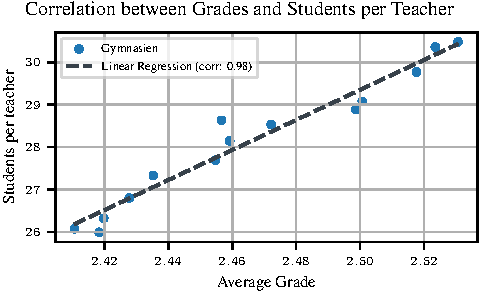
\includegraphics{fig/fig_correlation_grades_students_per_teacher.pdf}
    \caption{Linear regression on the students-to-teacher ratio by average Abitur grade. The resulting regression line (\textcolor{TUred}{\rule[-0.2ex]{0.5em}{2pt} \rule[-0.2ex]{0.5em}{2pt}}) is calculated over the aggregated average overall grammar schools (\textcolor{TUlightblue}{\tikz\draw[fill={TUlightblue}] (0,0) circle (0.25em);}) in Germany.}
    \label{fig:regression-stt-grade}
\end{figure}

As already explained, these results correspond only to grammar schools and are not necessarily representable for other schools or single federal states. Thus, the student-to-teacher ratio is also compared to the repeaters and the budgets per child in each federal state. Therefore, their Pearson correlation coefficients are calculated for each federal state across all years. 

\autoref{fig:heatmap_correlation_students_per_teacher_repeaters_budget} presents a visualization of the Pearson correlation coefficients, analyzing the relationship between the number of children per teacher and the average number of repeaters, as well as the educational budget per child. To visually represent the data across various federal states, a heatmap is generated. Therefore, the Pearson correlation coefficients for each state is normalized to the used color map scale. Consequently, each state a color representing the correlation coefficient is assigned. It is evident that there exists a strong positive correlation between the student-to-teacher ratio and the rate of repeaters in the most new federal states, while the correlation in the new federal states is significantly weaker. Moreover the correlation between the student-to-teacher ratio and the inflation adjusted budget per child tends to be positive for the new federal states and negative for the old federal states.

\begin{figure}[h]
    \centering
    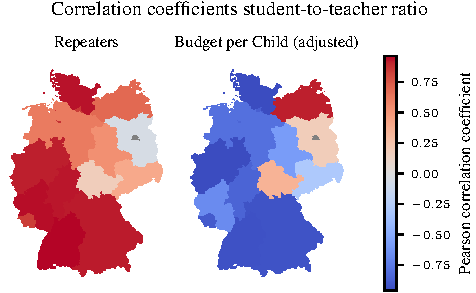
\includegraphics{fig/fig_heatmap_correlation_students_per_teacher_repeaters_budget.pdf}
    \caption{Pearson correlation coefficients between the student-to-teacher ratio and the relative repeater count (left) and the inflation-adjusted average budget per child (right). \textcolor{red}{Red} indicates positive, \textcolor{gray}{gray} neutral, and \textcolor{blue}{blue} negative correlations between the variables.}
    \label{fig:heatmap_correlation_students_per_teacher_repeaters_budget}
\end{figure}
